% main.tex

\section{Introduction}

In this section we give a brief history of the developments in the subject and an overview for the thesis.

\subsection{Brief history of the subject}

QCD is hard, $\N=4$ is easier. From Maldacena to Zarembo, Bethe ansatz, asyptotics, strings, algebraic curves, matching. Finally TBA, $\pmu$. Of course still a lot of things to do.

\vspace{20pt}
\newlength\yearposx
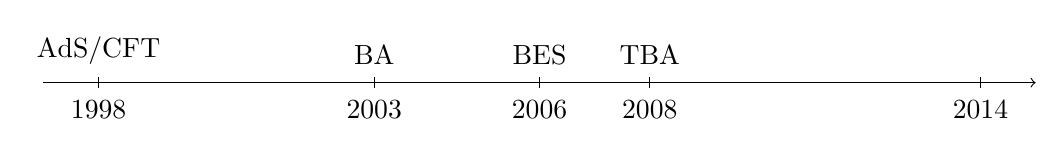
\begin{tikzpicture}[scale=0.70]
    % define coordinates (begin, used, end, arrow)
    \foreach \x in {1997,1998,2003,2006,2008,2014,2015}{
        \pgfmathsetlength\yearposx{(\x-1997)*1cm};
        \coordinate (y\x)   at (\yearposx,0);
        \coordinate (y\x t) at (\yearposx,+3pt);
        \coordinate (y\x b) at (\yearposx,-3pt);
		\coordinate (y\x r) at (\yearposx,-0.7pt);
    }
    % draw horizontal line with arrow
    \draw [->] (y1997) -- (y2015);
    % draw ticks
   \foreach \x in {1998,2003,2006,2008,2014}
        \draw (y\x t) -- (y\x b);
	% anotate
	\node at (y1998) [below=3pt] {1998}; \node at (y1998) [above=3pt] {AdS/CFT}; 
	\node at (y2003) [below=3pt] {2003}; \node at (y2003) [above=3pt] {BA}; 
	\node at (y2006) [below=3pt] {2006}; \node at (y2006) [above=3pt] {BES}; 
	\node at (y2008) [below=3pt] {2008}; \node at (y2008) [above=3pt] {TBA}; 
	\node at (y2014) [below=3pt] {2014}; \node at (y2014) [above=3pt] {$\pmu$}; 
        
\end{tikzpicture}

\subsection{Thesis overview}

Maybe a nice picture for the structure of the thesis.
